\section{Teórico}

  \definicion{Topic:} Density-functional perturbation theory (DFPT): phonons.

  \definicion{Speaker:} Stefano BARONI (SISSA, Italy).

\subsection{Funciones respuesta}

  Las funciones respuestas tienen la siguiente forma general
    $$propiedad = \frac{\partial variable}{\partial fuerza}$$

  donde \emph{fuerza} refiere a la fuerza de algún campo externo (eléctrico, magnético, de fuerzas/tensiones, etcétera).

  Permiten conocer tanto propiedades macroscópicas como microscópicas. En el caso miscroscópcio, la perturbación externa tiene el tamaño adecuado para lo que se pretende determinar.

\subsection{Teorema de Hellmann-Feynman}

  El ingrediente principal dentro de la teoría de funciones respuestas es el teorema HF.

  Pensémoslo primero en términos del Hamiltoniano y la energía. Supongamos que partimos de
    $$H_{\lambda} \Psi_{\lambda} = E_{\lambda} \Psi_{\lambda}$$

  donde el Hamiltoniano depende de un conjunto de parámetros externos ${\lambda}$ (aunque generalmente es una colección, puede ser un parámetro único), los cuales NO constituyen variables dinámicas. Luego, el teorema establece que
    $$\frac{\partial}{\partial \lambda} E_{\lambda} = \frac{\partial}{\partial \lambda} \expval{H_{\lambda}}{\Psi_{\lambda}}$$

  ya que el autovalor siempre puede pensarse como el valor de expectación del Hamiltoniano sobre los autoestados. Aplicando la regla de la cadena, se llega a
    $$\frac{\partial}{\partial \lambda} \expval{H_{\lambda}}{\Psi_{\lambda}} =
    \bra{\sfrac{\partial}{\partial \lambda} \Psi_{\lambda}} H_{\lambda} \ket{\Psi_{\lambda}} +
    \bra{\Psi_{\lambda}} \sfrac{\partial}{\partial \lambda}  H_{\lambda} \ket{\Psi_{\lambda}} +
    \bra{\Psi_{\lambda}} H_{\lambda} \ket{\sfrac{\partial}{\partial \lambda} \Psi_{\lambda}}$$
    $$= \bra{\Psi_{\lambda}} \sfrac{\partial}{\partial \lambda}  H_{\lambda} \ket{\Psi_{\lambda}} +
    E_{\lambda} \bra{\sfrac{\partial}{\partial \lambda} \Psi_{\lambda}} \ket{\Psi_{\lambda}} +
    E_{\lambda} \bra{\Psi_{\lambda}} \ket{\sfrac{\partial}{\partial \lambda} \Psi_{\lambda}} =
    \bra{\Psi_{\lambda}} \sfrac{\partial}{\partial \lambda}  H_{\lambda} \ket{\Psi_{\lambda}} +
    E_{\lambda} \frac{\partial}{\partial \lambda} \braket{\Psi_{\lambda}}$$

  Como los autoestados se suponen normalizados, tenemos que $\braket{\Psi_{\lambda}} = 1$ y, por lo tanto, $\frac{\partial}{\partial \lambda} \braket{\Psi_{\lambda}} = 0$. Se concluye entonces que
    $$\frac{\partial}{\partial \lambda} E_{\lambda} =
    \bra{\Psi_{\lambda}} \sfrac{\partial}{\partial \lambda}  H_{\lambda} \ket{\Psi_{\lambda}}$$

  Que la derivada del autovalor sea independiente de la derivada de los autovectores no es trivial: puedo avergiuar la derivada del autovalor con solo derivar el operador (y tomarle la media)!

  El teorema de HF se puede generalizar: es aplicable siempre que el problema se pueda escribir en términos de algún principio variacional. Supongamos que tenemos una función $g$ en función de un parámetro externo $\lambda$, la cual es el mínimo de un funcional $G$ que depende de una variable interna $x$ y el parámetro externo $\lambda$.
    $$g(\lambda) = \min_{x} G[x, \lambda]$$

  \Obs{En el caso de la energía nos quedaría
    $$E_{\lambda} = \min_{\Psi : \braket{\Psi}=1} \expval{H_{\lambda}}{\Psi}$$}

  El mínimos se encuentre derivando e igualando a cero: como $G$ depende de $\lambda$, el mínimo también depende de $\lambda$.
    $$\frac{\partial}{\partial x} G \Big|_{x = x (\lambda)} = 0 \Rightarrow g(\lambda) = G[x (\lambda), \lambda]$$

  Luego
    $$\frac{\partial}{\partial \lambda} g (\lambda) = \frac{\partial}{\partial x} G \Big|_{x = x (\lambda)} \frac{\partial}{\partial \lambda} x (\lambda) + \frac{\partial}{\partial \lambda} G \Big|_{x = x (\lambda)}$$

  Como estamos en el mínimo, sabemos que $\sfrac{\partial}{\partial x} G \Big|_{x = x (\lambda)} = 0$, con lo cual
    $$\frac{\partial}{\partial \lambda} g (\lambda) = \frac{\partial}{\partial \lambda} G [x, \lambda] \Big|_{x = x (\lambda)}$$

\subsection{Susceptibilidades: derivadas de la energía}

  La definición de susceptibilidad $\chi_{BA}$ es la derivada de un operador $B$ con respecto a un parámetro $\alpha$ que marca la fuerza de la perturbación. Se tiene que $A$ es una perturbación física mientras que $B$ es un observable.
    $$\chi_{BA} = \frac{\partial}{\partial \alpha} \expval{B}$$

  Supongamos que tenemos un Hamiltoniano que depende de una CL de perturbaciones $v_i$ con una contribución (fuerza) $\lambda_i$.
    $$H = H_0 + \sum_i \lambda_i v_i$$

  Luego la energía del sistema será
    $$E [\lambda] = E_0 - \sum_i f_i \lambda_i + \frac{1}{2} \sum_{ij} h_{ij} \lambda_i \lambda_j + ... $$

  donde la fuerza generalizada es $f_i = - \sfrac{\partial E}{\partial \lambda_i}$. Las derivadas primeras permiten determinar la optimización estructural y estudiar la dinámica molecular, mientras que las derivadas segundas $h_{ij}$ son funciones respuesta.

  Usando la nomenclatura de la teoría perturbacional, tenemos que
    $$f_i = - \expval{v_i}{\Psi_0} = - \int v_i (\vec{r}) \rho_0 (\vec{r}) d \vec{r}$$
    $$h_{ij} =  \int v_i (\vec{r}) \rho_j^{'} (\vec{r}) d \vec{r} = \int v_j (\vec{r}) \rho_i^{'} (\vec{r}) d \vec{r}$$

\subsection{DFPT}

  El potencial externo $V_{\lambda}$ actuando sobre el sistema lo podemos expandir según
    $$V_{\lambda} (\vec{r}) = V_0 (\vec{r}) + \sum_i \lambda_i v_i (\vec{r})$$

  Considerando cómo DFT define la energía y usando el teorema de HF se llega a que
    $$\frac{\partial^2}{\partial \lambda_i \partial \lambda_j} E (\lambda) = \int \frac{\partial}{\partial \lambda_j} n_{\lambda} (\vec{r}) v_i (\vec{r}) d \vec{r}$$

  Esta derivada segunada es la base de DFPT. Entonces para calcular la segunda derivada, debemos calcular la respuesta de la densidad de carga. Como $n$ es la suma sobre las normas cuadráticas de los autoestados KS, la derivada es sencilla de expresar. Usualmente los autoestados son reales, así que se peude olvidar la conjugación. Sin embargo a veces son útiles los estados de Bloch y ahí sí juega lo complejo.

  En DFPT lo que se hace es plantear un ciclo SCF análogoal de DFT y linealizar los 3 pasos (Fig. \ref{fig:DFPT}). Luego, se resuelve este nuevo ciclo SCF.

  \begin{figure}[H]
      \centering
      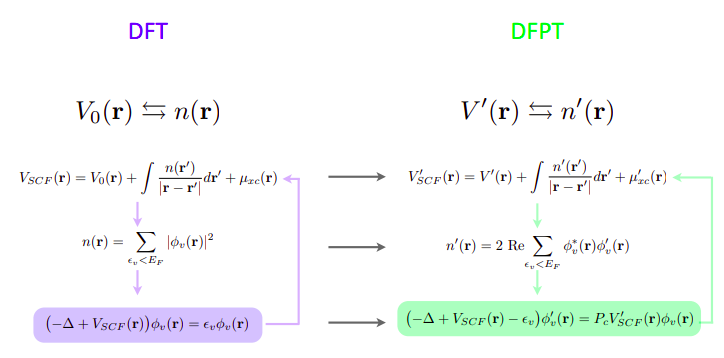
\includegraphics[scale = 0.6]{figs/D5/DFPT.png}
      \caption{DFT vs DFPT}
      \label{fig:DFPT}
  \end{figure}

\subsection{Simulación de vibraciones atómicas}

  Un cristal perfecto lo podemos describir como un potencial externo periódico (Fig. \ref{fig:red}). Queremos saber cuál es la respuesta del sistema respecto al desplazamiento individual de los átomos. A primer orden el potencial perturbativao es lineal en la amplitud de la distorsión atómica. Luego, para saber cómo depende la energía con la amplitud de la distorción, expandimos en Taylor y vemos que podemos pensarla directamente como curvatura o como derivadas primera de la fuerza. Esto se conoce como constante de fuerzas interatómicas (IFC) en el cotexto de la dinámica de redes.

  \begin{figure}[H]
      \centering
      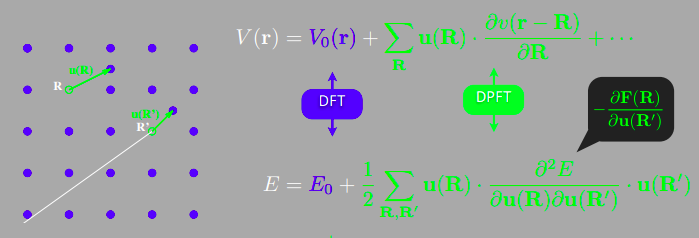
\includegraphics[scale = 0.6]{figs/D5/red.png}
      \caption{Dinámica de redes.}
      \label{fig:red}
  \end{figure}

  Ahora resolvemos la ecuación de autovalores para la matriz 3Nx3N de IFC (Fig. \ref{fig:vib}), la cual se conoce como matriz dinámica. Los autovalore son los cuadrados de las frecuencias vibracionales. Hay un factor $M$ que es la masa atómica, la cual puede incorporarse en el autovector.

    \begin{figure}[H]
      \centering
      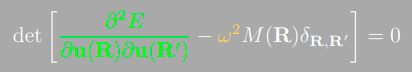
\includegraphics[scale = 0.6]{figs/D5/vibraciones.png}
      \caption{Problema de autovalores a resolver.}
      \label{fig:vib}
    \end{figure}

  Por la prueba de la derivada segunda, sabemos que el determinante tiene que ser positivo para asegurarnos que tenemos el mínimo. Esto se expresa con que los cuadrados de las frecuencias cuadradas tienen que ser positivas.

\subsection{Perturbaciones monocromáticas}

  Si queremos acomodar fonones de longitud de onda arbitraria, debemos hacer cálculos gigantes. Lo mejor es recurrir a la simetría: los fonones se clasifican en términos de sus números de onda. Los fonones de diferente longitud de onda no interactúan entre sí.

  Esto se refleja en DFPT al reescribir la longitud de onda en forma recíproca. Los orbitales no perturbados tiene vector de onda k definido (teorema de Bloch). Pero el fonon tiene vector de onda q. Entonces resulta que el número de onda general del resultado es k+q.

  Como el H es periódico, el KS orbital perturbado debe tener el mismo vector de onda (k+q): es un estado de Bloch. La densidad respuesta tiene el mismo número de onda que la perturbación. Lo mismo pasa con el potecial. Todo el cálculo puede mapearse entonces en calcular la parte periódica de la función de onda respuesta: la complejidad computacional del sistema yace en el número de electrones.

  \begin{figure}[H]
    \centering
    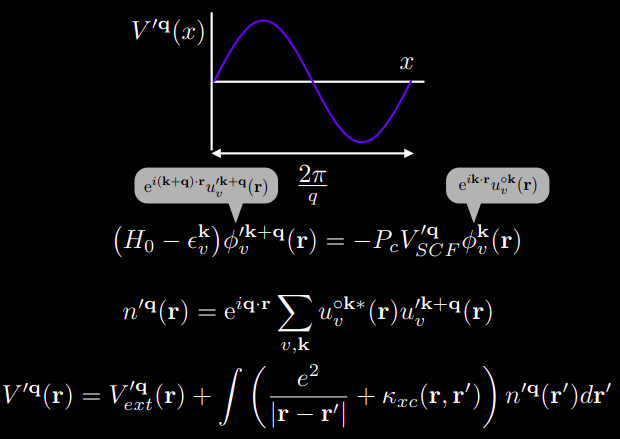
\includegraphics[scale = 0.6]{figs/D5/monocrom.png}
  \end{figure}

\subsection{Fonones en materiales polares}

  Generan un campo eléctrico macroscópico estos materiales. La energía depende de la distorción de red y del campo eléctrico. La parturbación tiene número de onda definido. El campo E es irrotacional en el espacio recíproco. En ausencia de cargas y corrientes: cuando la polarización del fonon es ortogonal a q, entonces la ecuación de Mawell se satisfce sólo cuando el campo es idénticamente nulo.

  Para los fonones transversales entonces la expresión es más sencilla. Ahora consideramos la otra ecuación de Mawell: se cumple sólo cuando D es nulo. Los fonones paralelos tienen otra expresión.

  Debemos tener una estimada de la carga efectiva y la constante electrica para calcular los fonones longitudinales.

  \begin{figure}[H]
    \centering
    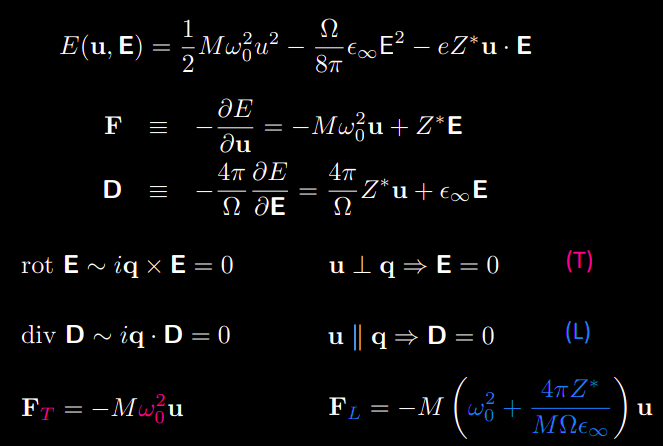
\includegraphics[scale = 0.6]{figs/D5/fonones_polares.png}
  \end{figure}

\subsection{Características principales DFPT}

  \begin{itemize}
    \item Calculo de funicones respuesta en términos de orbitales respuesta.
    \item Se resulven sistemas lineales sin calcular estados de conducción.
    \item Sólo se debe calcular la respuesta a la perturbación dada.
    \item También se pueden tratar perturbaciones no locales, no periódicas o campos eléctricos macroscópicos.
  \end{itemize}


\section{Q\&A}

  \definicion{Regarding acoustic phonons: how much is slightly different from zero? I mean when to consider it zero}

  It depends on the system and technicalities (xc functional, etc.). See point 7.2 here: https://www.quantum-espresso.org/resources/faq/phonons

  Let's say a few tens of $cm^{-1}$, more for lighter atoms (e.g. C), less for heavier atoms

  \definicion{does the enforcement of the acoustic sum rule shift every frequency at every q-point by the amount required by the first 3 modes at gamma? i.e., does it shift the whole phonon dispersion? or just the first 3 modes at gamma?}

  In principle, it should shift only the first 3 modes at gamma by a significant amount, all other modes by negligible amounts. If all modes change significantly after ASR, there is something not right.

  \definicion{Question: Is there a rule of thumb to choose the convergence criteria (conv\_thr) in scf.in input and (tr2\_ph) in ph.in . Which psuedopotential (norm-conserving or ultrsoft)  do you recommend to avoid having imaginary frequency.}

  For geometry optimizations I typically use conv\_thr = 1e-9 to 1e-10 (if the system converges that far), but instead of specifing conf\_thr=1e-9, I specify conf\_thr =1-e7 and upscale = 100.

  Note that conv\_thr is extensive and depends on the number of atoms, e.g. for 10x more atoms, multiply conv\_thr by 10.
  As for the tr\_ph: it is analogous to conv\_thr, but notice that it is a "square", hence conv\_thr =1e-8 would corresponds to tr2\_ph = 1e-16.

  Type of  pseudopotential have nothing to do with imaginary frequencies.

\section{Hands-on}

  \definicion{Topic:} DFPT.

  \definicion{Speaker:} Andrea URRU (ETH, Switzerland), Iurii TIMROV (EPFL, Switzerland).

\subsection{Introducción}

    Vamos a calcular la fono freq y fonon disp.

    Ver conceptos básicos.

    usa: alfa comp desplazamiento del átomo s (son 3xN) autovec

    La cantidad de fonon's freq que obtenemos es 3N.

    El concepto central: interactomic force Constantes

    Habla cómo llega al problema de autovaores. Lo que queremos diagonalizar es la matriz dinámica. Los autovalores son las freq fonónicas. Los autovectores están asociados (no son) los atomc displac (están divididos por la raiz de la masa atómica). De ahí se saco la masa que había en el teórico!

    El código de fonones cover gran variedad de sistemas y métodos: ver listado.

\subsection{Ex 1a}

  ASR ver filminas! (13, 14, 15)


  Nonpolar material (silicon).

  Debemos resolver un sistema lineal que nos permite derivar primera de las funciones de onda. Pero a la derecha había otra cosa. Clave: los orbitales KS de ground state. Por eso es que necesitamos correr primero el pw.x.

  Input de ph.x: al final se pone el vector de onda particular que se quiera calcular. Vemos que el umbral es bajísimo: es una derivada segunda! (a la -14).

  La matriz dinámica se guarda en fildyn, que es lo que después se va a usar.

  ph.x output: como en la Si tenemos dos átomos en la elda unidad, tendremos 6 modos fonónicos. Se resuelven a tres por simetría. (de a 3 mods). Cuando ddv\_scf\^2 es menor que le umbral que dimos en el input, se considera alcanzada la convergencia. Luego de la convergencia se encuentran las frecuencias.

  Vemos que hay 3 freq neg: indican que el cuadrado de la freq es negativa. Se tienen frecuencias imaginarias. Sería un signo de inestabilidad.

  Se pede ver que en este caso justo corresponde a ruido numérico, porque son negativas, pero muy cercanas a cero. (ver la presentación).

  Los modos acusticos en gamma deberían ser necesariamente nulos. Debido a que la freq fononica está dada por diferenias en energía originadas por la distorsion fononica. (algo mas). Como los modos acusticos en gamma son traslaciones rígidas. Por la invariancia traslacional, la energía del sistema es invariante y por eso la freq es nula.

  Habla de la regla de la suma acustica. Hay una condicion de la invarianza traslacional. Esta condicion no es impuesta por deefault. Este cero  pero no ser un cero en términos numéricos.

  El dynmat.x viene a corregir esto me parece que entendi. revisar. Esto impone la suma del gammma de no se quien.

  El dynmat.out contiene las freq de la matriz dinámica corregida. Ahora lo que es cero, realmente es cero.

  Los otros 3 modos son los modos ópticos.

  Por qué no se hace automáticamente? no hay por qué. En realidad es una cuestión de cálculo del R-espacio.


  You inspect the phonon dispersion and check if you have negative frequencies. There can be two reasons: 1) physical - the system is dynamically unstable, 2) numerical - your results are not converged


\subsection{Ex 1b}

  Interpolación de Fourier (ver filminas 26). Permite interpretar como la smooth fonoo dispersion es calculada en el QE.

  En vez de calcular punto a punto (muy caro sobre todo si nos vamos fuera de gamma por la pérdida de simetrías). Lo que se hace es una técnica de interpolación. Se calcula en una coarse k-mesh.

  Se llama de Fourier porque la interpolación necesita ir y volver entre espacios duales. Hacemos la FT de la matriz dinámica con una k-mesh gruesa. Esto nos da una idea de la interatomic force constanst sobre todo el espacio real. Luego hacemos una FT de regreso, pero podemos pedir el punto que se nos cante: tener 10 puntos de inicio y después pedirle 100. No importa la simetría.

  Los nuevos puntos estána a lo largo de las líneas de alta simetría.

  q2r.x hace la transformacion de ida hacia el real y matdyn.x nos trae de vuelta al recíproco. En este aso la ida era sobre 8 puntos, pero la vuelta es de 396.

  ldisp = .true.,
  7   nq1 = 4,
  8   nq2 = 4,
  9   nq3 = 4,

  le dice que queremos una dispersion fononica con una mesh 4x4x4.

    ph.si.out vemos que hace todo el cálculo de antes pero para cada uno de los 8 puntos de la mesh (cuales 8?)

  En los Si.dyn se tiene la matriz dinamica para cada uno de los puntos.

  Cómo saber que estamos usando una grilla gruesa lo suficientemente fina? Hacer pruebas. Corroborar visualmente si hay cambios muy graves. Comparar 2x2x2 4x4x4 6x6x6 8x8x8. Hacer plotban para cada grilla. Incluir lo que falta.

  Otra manera es hacer un cálculo directo. Como es una interpolación, se puede hacer una single q vector calculation. Calcular algunitos y ver que caigan sobre la curva generada con la mesh dada.

  Cualquiera de las dos va a andas bien.

  Hw2: ver filmina.

  Phonon mode visualizer: ver filmina. Lee directamente el input del pw y el ouput "matdyn.modes". Tocas interactivamente los modos fonónicos y te muestra cómo se van moviendo. También podes ver la celdad unidad para entedner cómo el desplazamiento fonónico son modulados por el q vector.

  Ver cuando la interpolación ya no funciona tan bien (filmina).

  IFC Interatomic Force Constants.

\subsection{Ex 2a}

  Aislantes polares: aparece una contribución no analítica. Hay dos valores que neceisto Z epsilon. debo caluclar con campo elecrico.

  input del ph.x
  epsil = .true.
 hace el calculo con el campo eéctirco eso que hace falta

  todavía no le pusimos la parte del polar insulatro. Sólo esamos calculando un aparte (Ver cual era). No aparecen las separaciones LO-TO: las 3 freq opticas están degeneradas dada la simetría del sistema. Cuadno se incluye le termino no analitico, aparece spliting. (efecto stark?)

  dynmat ahora le especificamos los vecotres que sacamos (las que no están en la parte analitica). Al no ser analitica debemos decirle a direccion d aproximacion.
  q(1) = 1.0,
  7     q(2) = 0.0,
  8     q(3) = 0.0

  Vemos que despues de esto se levanta la degeneración: LO-TO splitting se llama esto.

\subsection{Ex 2b}

  Faltan cosas en todos los inputs. Están comentadas las líneas faltantes. Tratar de hacerlo solitos Bb. Análogo al 1b.

  Al acercarnos a gamma tenemos el splitting LO-TO.

\subsection{Ex 3}

  Hacer el ex3 solos tambien

  No trabaja con 20 procesores. Sí trabaja con 8.


  ver los libros sugeridos. Uno es el cenizas para lo general y otro es de FOx para lo de la separacion LO-TO.

----

La carpeta que borre que "estaba vacía" en relidad tenía archivos ocultos!! son las configuraciones y gilada que robe de la VM.
